\chapter{PROPOSED SOLUTION}
\label{chap:solution}

This chapter describes the proposed solution which is a system consists of two subsystems: A crowd-sourcing system and an analysis system. In \textit{Requirement analysis and System overview} subsection, everything is briefly described as a whole. In two last sections, structure and details of two subsystems are defined more comprehensively.

\section{Requirement analysis and system overview}
\subsection{Requirement analysis}

To be able to utilize data to serve a security purpose, the most obvious method would be to analyze visual data such as photos and videos, and the current most effective way to do so is using Artificial Intelligence. In recent years, advancements in Artificial Intelligence, especially in Neural Networks, significantly enhanced the development of computer vision field. On the famous ImageNet \footnotetext{Source: \url:{http://www.image-net.org/challenges/LSVRC/}} dataset, trained neural networks can now generate results that are better than human in classifying images (Figure \ref{chap3:deeplearning_vs_human}). 

For Deep learning models to be successful, sufficient training data must be provided. \cite{DBLP:journals/corr/SunSSG17} Found out that the effectiveness of computer vision related tasks scales logarithmically with the amount of training data. Regardless of the importance of data in Deep learning models, there are few to none security datasets that are suitable for the environment of Vietnam. 

\begin{center}
    \begin{figure}[H]
    \centering
    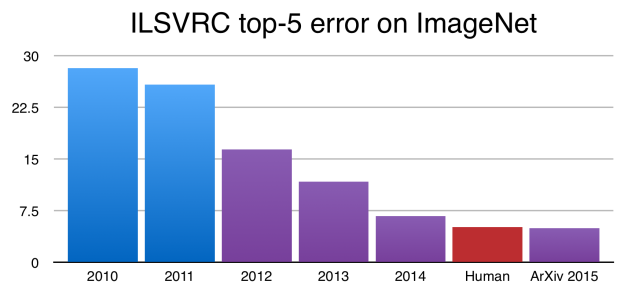
\includegraphics[width=0.75\columnwidth]{images/chap3/deeplearning_vs_human.png}
    \footcaption{Neural Network out-performing human in 2015 on ImageNet Large Scale Visual Recognition Challenge}
    \label{chap3:deeplearning_vs_human}
    \end{figure}
\end{center}
\footnotetext{Source: \url:{ https://devblogs.nvidia.com/mocha-jl-deep-learning-julia/}}

A traditional method of collecting data would be to set up an array of cameras at desired locations and then obtain their recordings. Those recording would later be labeled by specialists or experts and processed to form a dataset. This way of doing is expensive and require a lot of human resources. 

One other method of data collection is to implement Web crawler to pull data from the internet automatically. This method would be most useful for getting a large amount of data given a keyword. One downside is that data achieved by this method often contain considerable noise because of typos, mislabel or error. In the context of security, those data are not suitable for used because they are incredibly diverse and do not portray the Vietnamese environment accurately. 

Crowdsourcing is also one of the effective methods of data collection that is becoming a trend in the last couple of years. The idea behind crowdsourcing data is to build datasets with the help of a large group of people. An example of this kind of model is Wikipedia\footnotetext{\url:{https://www.wikipedia.org}}
. Wikipedia is an enormous web-based, collaborative encyclopedia which has over 100,000 volunteers contributing new information to the system daily. The success of Wikipedia proves that people can contribute to a system without profit. 

However, how can people be encouraged to provide their knowledge and information? Interaction with others is proven successful in increasing engagement of people, as Social media has been a popular trend among Vietnamese in recent years. At the time of November 2018, the amount of people using Facebook has reached about 70 million, that accounts for almost 73\% of the population. (Figure \ref{chap3:social_media_vn}).

Because of the reasons above, this thesis proposes building a \textbf{Social media platform for security}. This platform serves as a place where users can interact with each other, as well as allows people to contribute their knowledge to the system via crowdsourcing.  
\begin{center}
    \begin{figure}[H]
    \centering
    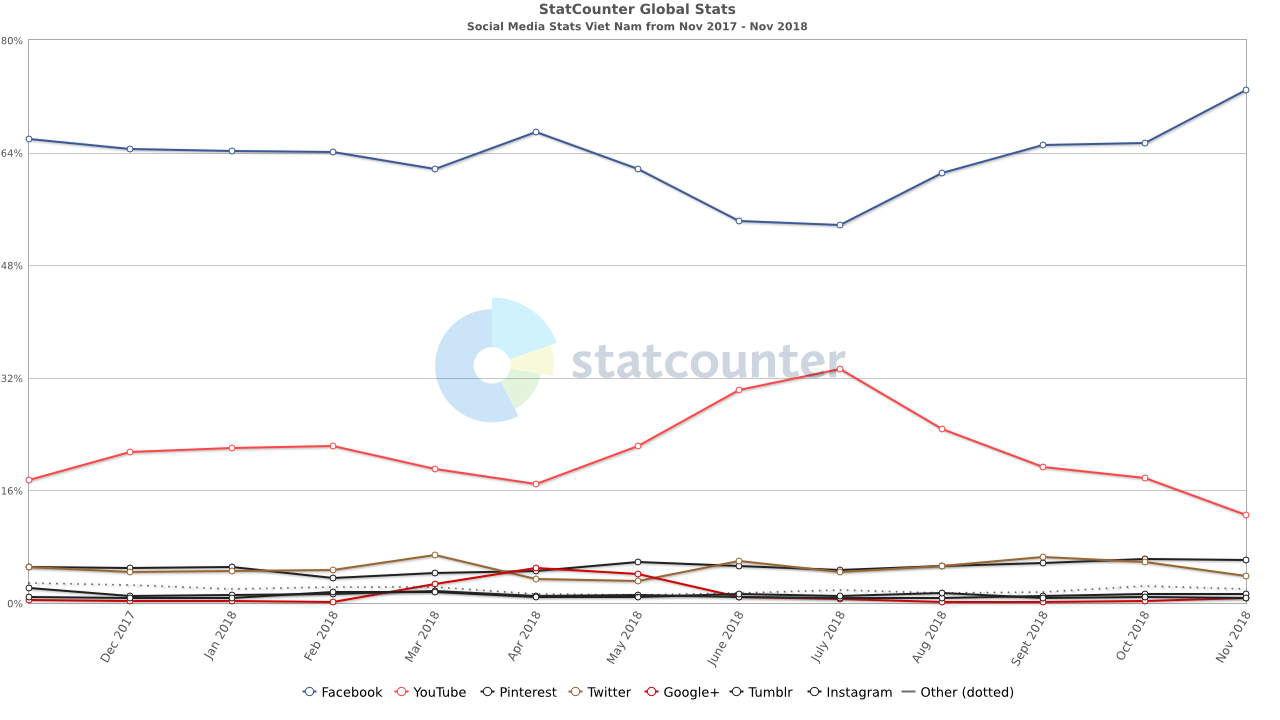
\includegraphics[width=1\columnwidth]{images/chap3/social_media_vn.png}
    \footcaption{Social media usage of Vietnamese is at all time high. Nearly 73\% of the population is using use Facebook}
    \label{chap3:social_media_vn}
    \end{figure}
\end{center}
\footnotetext{Source: \url:{http://gs.statcounter.com/social-media-stats/all/viet-nam}}

Figure \ref{chap3:system_overview_basic} shows a concise overview of how the system operates. Users interact with the \textbf{Crowd-sourcing system} through \textbf{User Interfaces}. The input of users can come in the form of images, videos or label contribution and are stored in the database. The system is also responsible for obtaining appropriate contents from the database to display to users through user interfaces.

\begin{center}
    \begin{figure}[H]
    \centering
    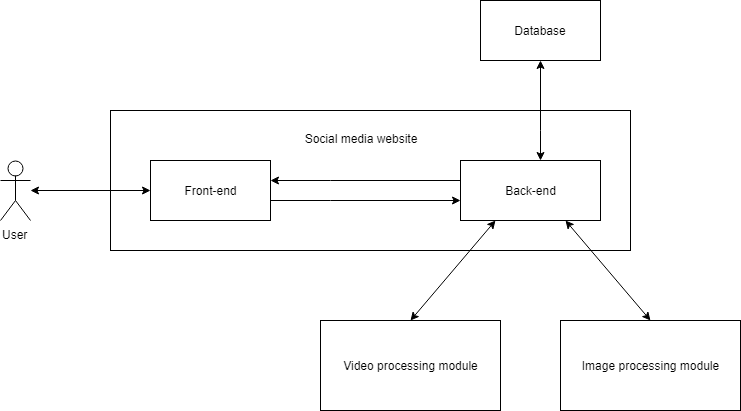
\includegraphics[width=1\columnwidth]{images/chap3/system_overview_basic.png}
    \caption{An overview of the system}
    \label{chap3:system_overview_basic}
    \end{figure}
\end{center}

Whenever there are videos to analyze, the server will send them to the \textbf{Video classifier module}, then get results back. Results returned from video classifier module are classified activity from the video and frames that contain faces in them. \textbf{Face Recognition module} does the job of identifying people in images. Results of both \textbf{Video classifier module} and \textbf{Face Recognition module} are used to determine security threats each video or image shows.
\section{Crowd-sourcing system}
\subsection{Database}
The project database divides into two different parts: \textbf{Cloud storage} and a \textbf{NoSQL database}. Why it requires such a complex system? The primary target is to reduce website loading time. Let take an example, if files are stored directly on the crowd-sourcing server. When many users request a file simultaneously, the server with limited bandwidth will cause delay. “53\% of mobile site visitors leave a page that takes longer than three seconds to load” – \href{https://think.storage.googleapis.com/docs/mobile-page-speed-new-industry-benchmarks.pdf}{Google}. What if these files stored on cloud storage? The client will be served by the cloud storage provider, which has higher availability.
\section{Analysis system}
The project requires two systems for analysis: A face recognition system and a video classifier system. The facial recognition system takes pictures of human faces as input and returns their identification. The video classifier system analyzes videos to find out actions in them. The remaining of this section describes in detail about the two analysis system.
\subsection{Face recognition module}
\subsection{Video classifier module}
Video classifying is not a new task in the field of Deep learning.
	



